\documentclass{article}
\usepackage{graphicx} % Required for inserting images

\title{Práctica de Laboratorio 4: Layouts}
\author{Yoel Nhelio Canaza Chagua}
\date{September 2024}
\usepackage{hyperref}
\usepackage{float}

\usepackage{geometry}
\newgeometry{left=3cm, right=3cm, top=2.5cm, bottom=2.5cm}

\begin{document}

\maketitle

\section{Enunciado de la tarea}

\begin{figure}[H]
    \centering
    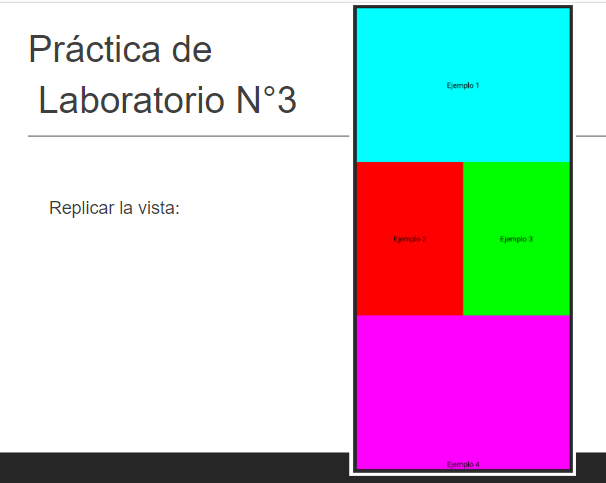
\includegraphics[width=0.5\linewidth]{1.png}
    \caption{Enunciao de la tarea}
    \label{fig:enter-label}
\end{figure}

\section{Vista replicada}

\begin{figure}[H]
    \centering
    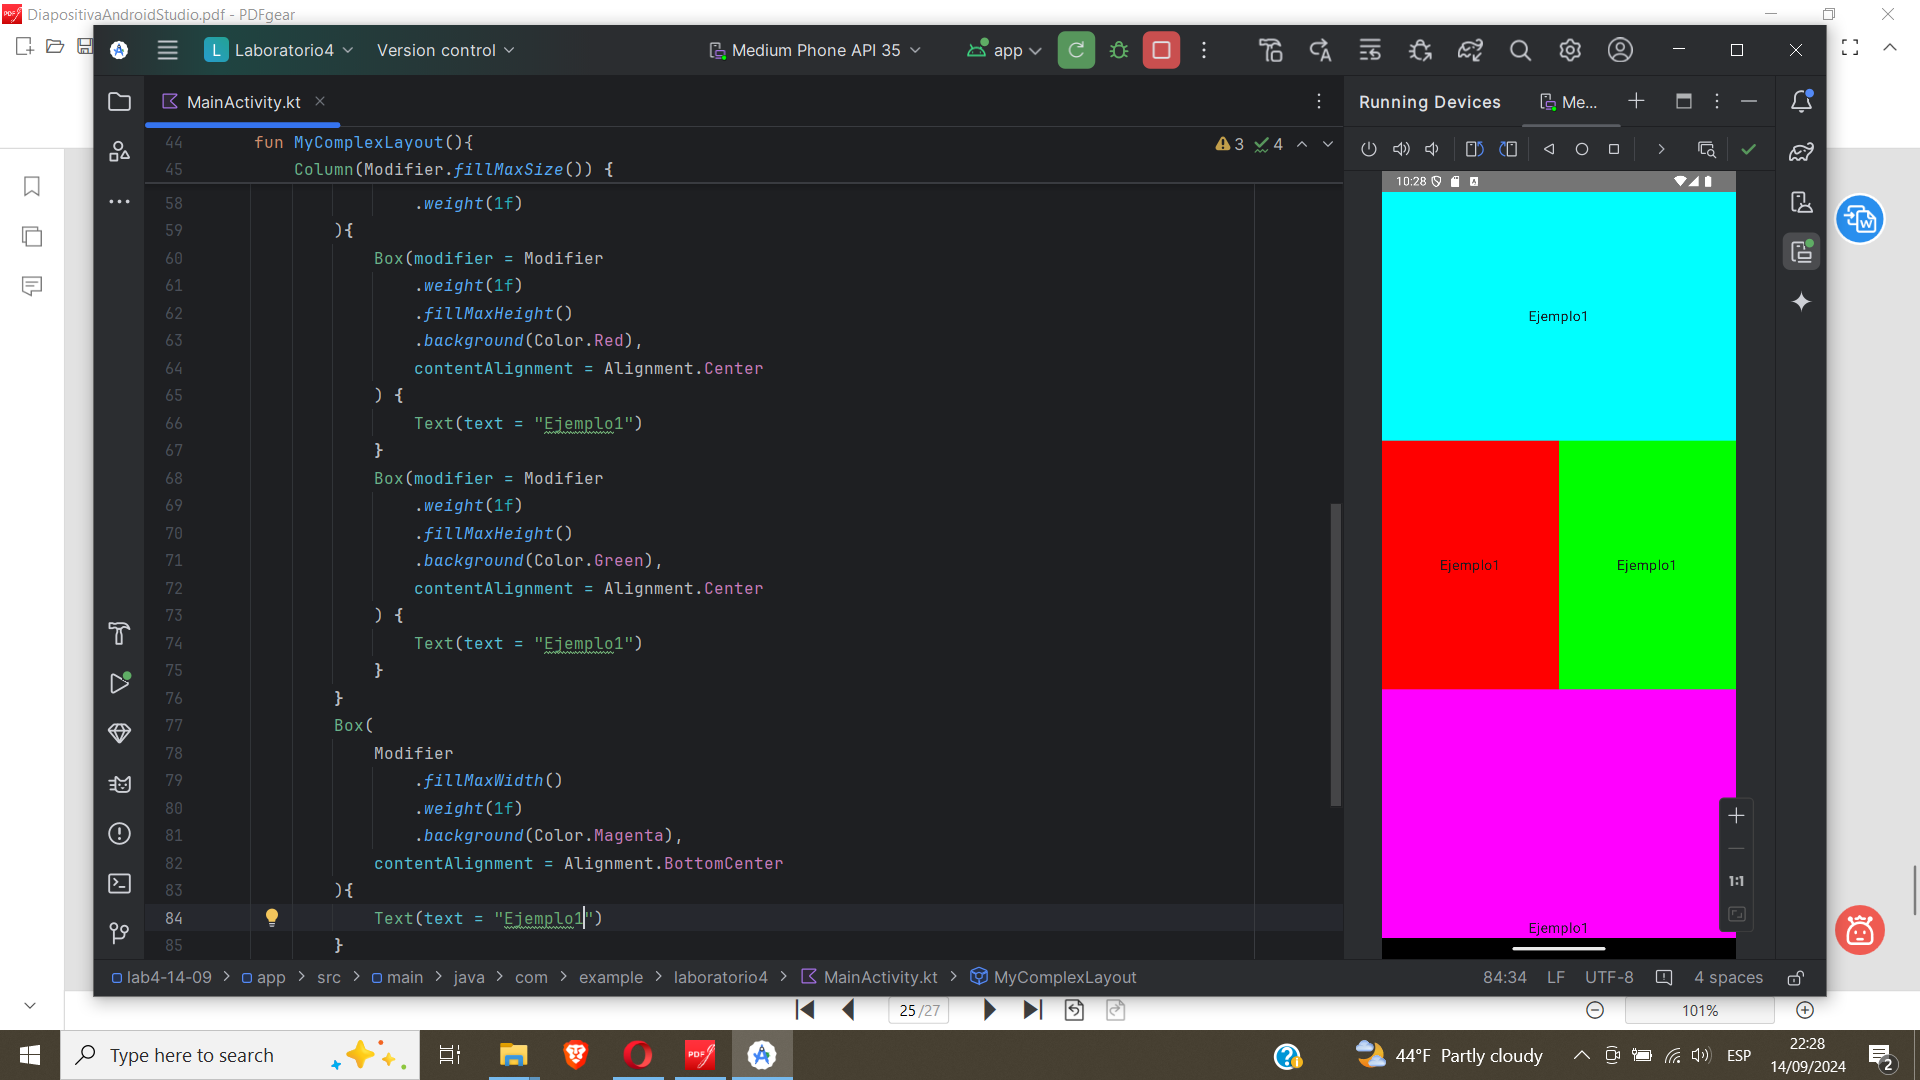
\includegraphics[width=0.8\linewidth]{2.png}
    \caption{Vista replicada}
    \label{fig:enter-label}
\end{figure}


\section{Prueba extra}

\begin{figure}[H]
    \centering
    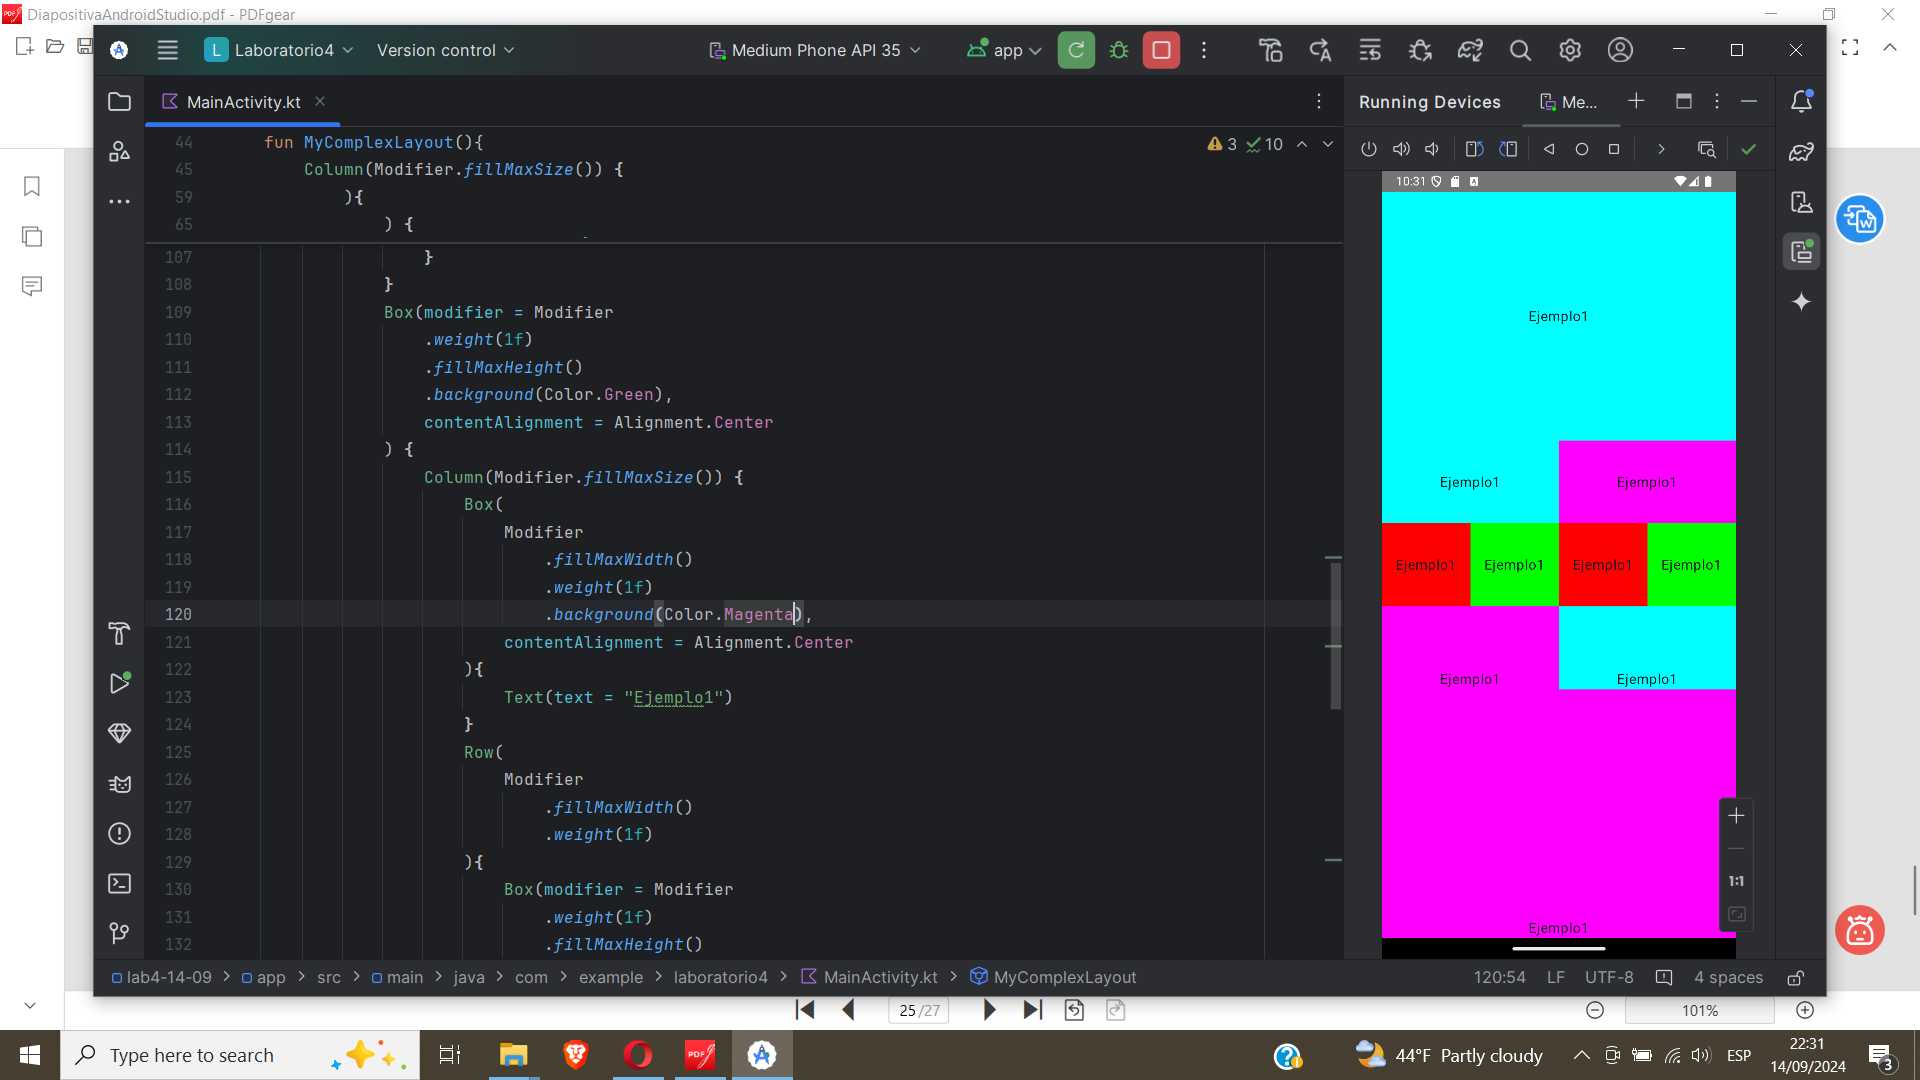
\includegraphics[width=1\linewidth]{3.png}
    \caption{Pruba extra}
    \label{fig:enter-label}
\end{figure}

\section{Anexos}

El código de la práctica se puede encontrar en el siguiente enlace (sólo se incluyó el código de MainActivity.kt:

\href{https://github.com/YoelCanaza/UniversityProjects/blob/c53c0969b7d803a3e589fa0b6541304063ea60f4/Desarrollo%20Basado%20en%20Plataformas%20II/Pr%C3%A1cticaLaboratorio4/MainActivity.kt}{Código MainActivity.kt}

También se puede ver el archivo en LaTeX en el siguiente enlace:

\href{}{Archivo en LaTeX}



\end{document}
